\documentclass{article}
\usepackage[utf8]{inputenc}
\usepackage{graphicx}


\begin{document}

\section{Connexion à Office 365 et Teams}

Nikolai

\section{Apparence de la page d'accueil}

La page d'accueil de Teams se présente sous forme d'une liste de classes 

\begin{figure}[h]
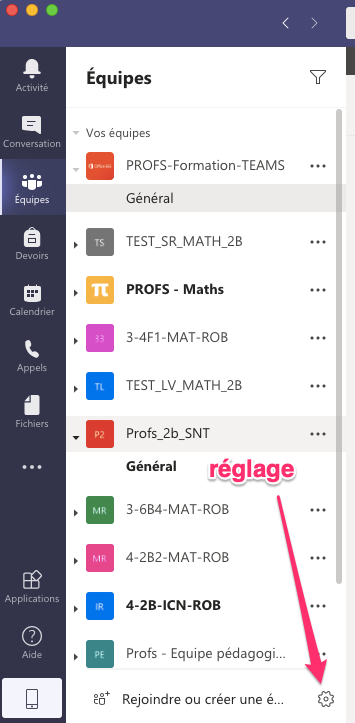
\includegraphics[width=2.5cm]{accueil_liste.png}
\centering
\end{figure}

ou sous forme d'une grille de classes 

\begin{figure}[h]
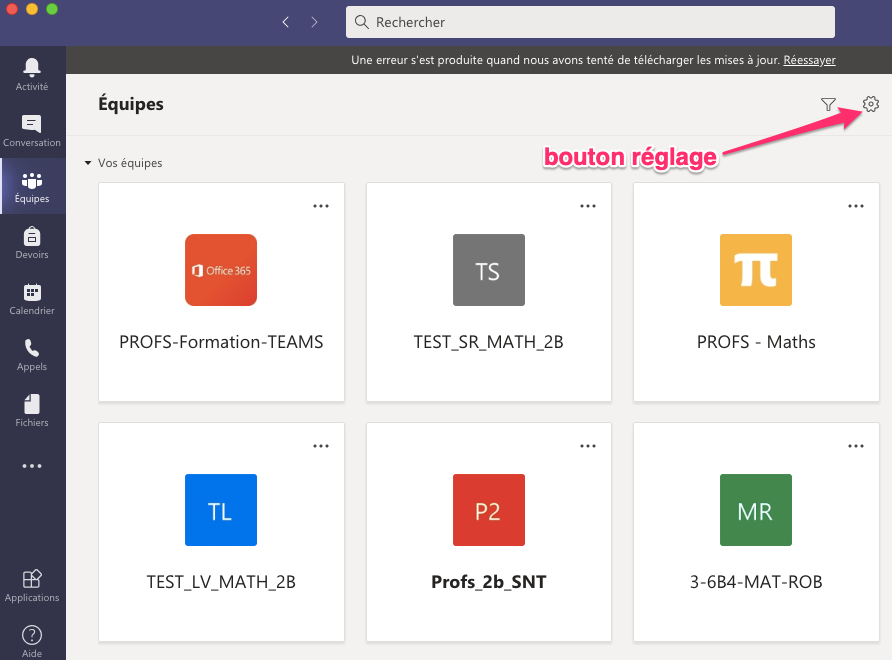
\includegraphics[width=5cm]{accueil_grille.png}
\centering
\end{figure}

Pour passer d'une forme à l'autre, il faut cliquer sur le sigle 
\includegraphics[width=0.7cm]{bouton_parametres.png}, choisir \textit{Changer d'affichage} dans le menu déroulant, comme dans l'exemple illustré ci-dessous :

\begin{figure}[h]
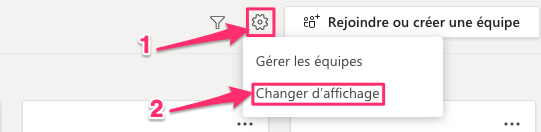
\includegraphics[width=5cm]{changement_liste.png}
\centering
\end{figure}

il faut ensuite sélectionner le type d'affichage souhaité entre \textit{Grille} et \textit{Liste}

\begin{figure}[h]
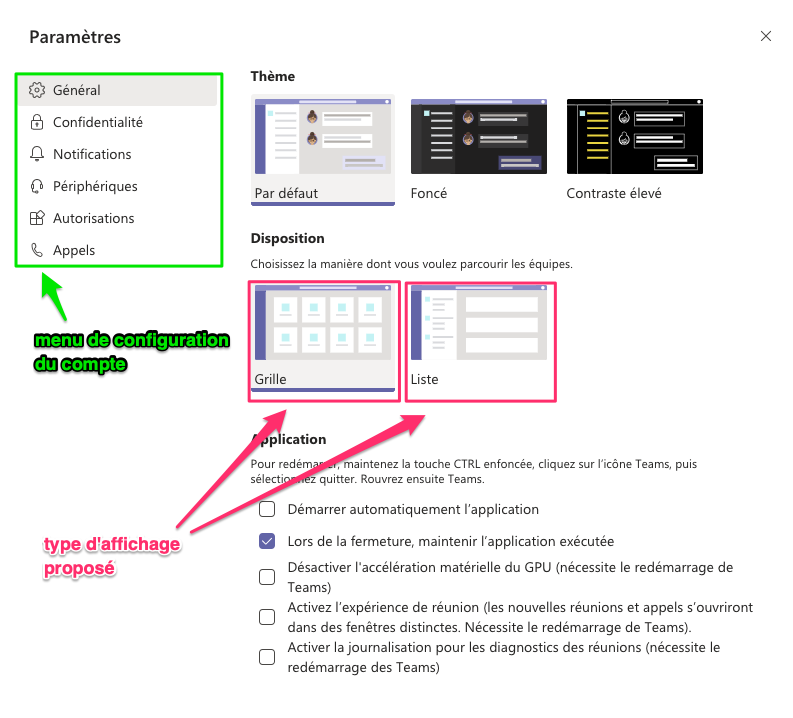
\includegraphics[width=10cm]{choix_parametre.png}
\centering
\end{figure}

 rajouter l'entrée dans la classe

\section{Utilisation de la messagerie}

\section{Consulter un document déposé par l'enseignant}

\section{Déposer un devoir}

Pour consulter les devoirs déposés par votre enseignant, il faut choisir \textit{2 de plus} dans la barre de menus du haut de page, puis sélectionner \textit{Devoirs}

\begin{figure}[h]
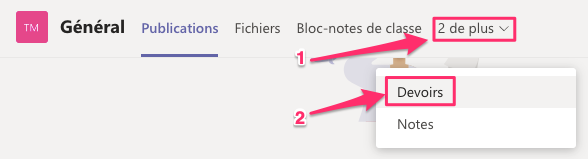
\includegraphics[width=8cm]{devoir1.png}
\centering
\end{figure}

La page qui s'affiche maintenant fait le bilan de ce qui a déjà été fait et des devoirs déposés par votre enseignant.

\begin{figure}[h]
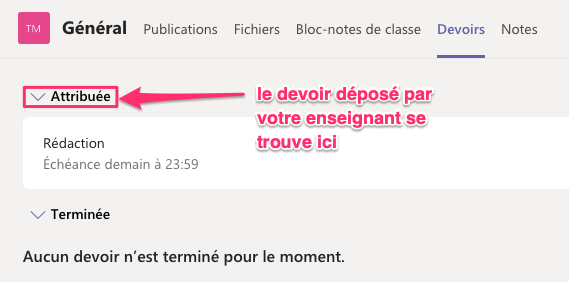
\includegraphics[width=8cm]{devoir2.png}
\centering
\end{figure}




\end{document}